
%***********************************************************************

% This is a template to be used for the preparation of
% papers submitted to the 34th International Workshop on
% Statistical Modelling, to be held in Trieste, Italy,
% July 18-22, 2022.

% Please follow the following general guidelines:
%
% (1) Do not specify any definitions, commands or style parameters.
%     Upon submission, your file will be checked for presence of
%     \newcommand or \def statements and if found, error message will be reported
%     by the submission form.
%
% (2) Follow the template below very tightly.
%
% (3) Include .pdf figures using the \includegraphics
%      command, an example of which are given below.
%
% (4) Use file names which begin with the surname of the first author.
%
% (5) When creating labels for cross-references, please start always
%     by surname of the first author, e.g., \label{smith:likelihood}
%
% (6) The template below contains some example materials
%      to guide you through the preparation of your paper.  However,
%      remove all the redundant material from your final document
%      before submitting.

% The guidelines above are needed in order to be able to combine all
% the papers into a single proceedings book of acceptable quality.
% Please follow the guidelines as strictly as possible. Deviations may
% result in papers being either refused by the registration form
% or sent back to the authors with the request to change
% their documents according to the guidelines.

% Special characters:
% Please do not use special characters (e.g., accents).
% Use TeX composition instead, such as \~n, \'a, \`e, \v{s}, \r{u} etc.

% Changes as of IWSM 2013:
%  * \usepackage{booktabs} added which allows \toprule et al. in the tabular environment
%    (\hline\hline is not longer used)
%  * '^\T' added in iwsm.sty to denote transposed vectors and matrices within math (see example below)
%  * \usepackage{amsmath, amssymb} introduced since IWSM 2012 is allowed (allowing usage of boldsymbols
%    and other handy constructions (align, pmatrix etc.) within math)
%  * \usepackage{psfrag} introduced since IWSM 2012 is NOT allowed
%
%

%***********************************************************************
% PLEASE LEAVE THIS PART UNCHANGED
%***********************************************************************

\documentclass[twoside]{report}
\usepackage{iwsm}
\usepackage{graphicx}
\usepackage{amsmath, amssymb}
\usepackage{booktabs}

% Please do not specify any new definitions, any new commands,
% and do not specify any style parameters.
% The preamble of the document should be left unchanged.

\begin{document}
	
	%***********************************************************************
	% PLEASE INSERT YOUR CONTENT FROM HERE
	%***********************************************************************
	
	% Title and running title to be used as left header:
	\title{The Feature-First Block Model}
	\titlerunning{The Feature-First Block Model}
	
	% Authors and running list of authors to be used as right header:
	\author{Lawrence Tray\inst{1}, Ioannis Kontoyiannis\inst{2}}
	\authorrunning{Tray and Kontoyiannis}    %% use \authorrunning{Surname 1} if only 1 author
	%% use \authorrunning{Surname 1 and Surname2} if two authors
	%% use \authorrunning{Surname 1 et al.} if more than two authors
	
	% Institutes of all authors
	% Include city and country of each institute, do not include the full address.
	\institute{Department of Engineering, University of Cambridge, UK
		\and Statistical Laboratory, University of Cambridge, UK}
	
	% E-mail of presenting author for correspondence
	\email{lpt30@cantab.ac.uk}
	
	% Brief abstract of the paper:
	\begin{abstract}
	Labelled networks are an extremely common and important form of data. A typical inference goal is to determine how the vertex labels (called features) affect graphical structure. The standard approach to this problem is to partition the network into blocks grouped by distinct values of the feature of interest. We then use a block-based random graph model - typically a variant of the stochastic block model (SBM) - to test for evidence these extracted feature-based communities interact differently with one another.
	
	Nevertheless, these feature-based communities are often not a natural partition of the graph and thus the model is not a good fit. With this in mind, we present a novel generative model, which we call the feature-first block model (FFBM), for better describing vertex-labelled undirected graphs. We present a method to efficiently sample the FFBM parameters. This allows us to automatically determine which features best explain the block-based graphical structure. Importantly, this analysis can be performed using the whole feature-set rather than considering each feature independently. 
	
	We apply the developed method to a variety of network data to extract the most important features along which the vertices cluster. Those that do not impact the high-level structure can be discarded to reduce the problem dimension. In the case the vertex features available do not readily explain the community structure in the resulting network, the approach detects this and is protected against over-confidence. Future work may benefit from extending the FFBM to multiple hierarchical levels. This allows the structure to be explained at each level of coarseness. 
\end{abstract}
	
	% Keywords (at most 5):
	\keywords{Stochastic Block Model; Labelled Networks; Inference.}
	
	% Produce the title:
	\maketitle
	
	% Main text
	\section{Introduction}

Many real-world networks exhibit strong community structure, with most nodes belonging to densely connected clusters. 
In this work, we examine vertex-labelled networks, 
referring to the labels as {\em features}. A typical goal is to determine whether a given feature impacts graphical structure. Answering this requires a random graph model;
the standard is the stochastic block model (SBM) -- see Peixoto (2017).

Analysing a labelled network with a simple SBM variant, requires partitioning the graph into blocks grouped by distinct values of the feature of interest. The associated model can then be used to test for evidence of heterogeneous connectivity between the feature-grouped blocks. Nevertheless, this approach can only consider disjoint feature sets and the feature-grouped blocks are often an unnatural partition of the graph.

We would instead prefer to partition the graph into its most natural blocks and then find which of the available features -- if any -- best predict the resulting partition. Thus motivated, we present a novel framework for modelling labelled networks.
This is not the first extension of the SBM to labelled networks, e.g. Stanley et al (2019). However, most of the current approaches are focused on leveraging feature information to partition the graph more reliably in the presence of noise.
We seek instead to develop a model well suited for inferring how vertex features impact graphical structure and to report our confidence in those conclusions.

	
	%\section{Preliminaries}

This section defines some preliminary concepts required for the subsequent analysis. We first need a model for community-like structure in a graphical network. For this we adopt the stochastic block model (SBM) - widely used across academia. The premise is that each node in the graph belongs to a unique community called a block. The probability that two nodes are connected depends only on the block memberships of each. Graphs drawn from the SBM ensemble exhibit community structure. Specifically, we will use the microcanonical variant of the SBM, proposed by \citet{Peixoto-Bayesian-Microcanonical}. A paraphrased definition is given below for the non-degree-corrected SBM (NDC-SBM).

\begin{definition}[Microcanonical NDC-SBM]
	\label{defn:microcan-ndc-sbm}
	Let $N \in \Integers^{+}$ denote the number of vertices in an undirected graph. The block memberships are encoded by a vector $b$ of length $N$ where each entry $b_i \in \{1, 2 \dots B\}$. $B \in \Integers^{+}$ is the number of non-empty blocks. Let $e$ be a $B \times B$ matrix of edge counts between blocks ($e_{rs}$ is number of edges from block $r$ onto block $s$ - or twice that number if $r=s$). For undirected graphs $e$ is symmetric. For a non-degree-corrected stochastic block model (NDC-SBM), we say that the graph $A$ is generated as follows:
	%
	\begin{equation}
		A \sim \textrm{NDC-SBM}_{\textrm{MC}} (b, e)
	\end{equation}
	%
	Where edges are placed uniformly at random but respecting the constraint imposed by $e$ and $b$. The additional parameters $N$ and $B$ are omitted as they are inferred from the shapes of $b$ and $e$. If we interpret $A$ as an adjacency matrix, then this constraint can be written formally as: $e_{rs} = \sum_{i,j} A_{ij} \one \{b_i = r\} \one \{b_j = s\}$.
\end{definition}

Nevertheless, this formulation does not accept high degree variability within blocks as is typical of real-world data. Indeed, the NDC-SBM favours a partition into high-degree and low-degree nodes rather than clusters of inter-connected nodes. We therefore introduce the degree-corrected SBM (DC-SBM) \cite{Peixoto-Bayesian-Microcanonical} to circumvent these issues. 

\begin{definition}[Microcanonical DC-SBM]
	\label{defn:microcan-dc-sbm}
	This is much like the NDC-SBM but has an additional parameter $k$ which is an $N$-length vector encoding the degree sequence ($k_i$ is the degree of vertex $i$). Therefore, we write:
	%
	\begin{equation}
		A \sim \textrm{DC-SBM}_{\textrm{MC}} (b, e, k)
	\end{equation}
	%
	Once again, edges are placed uniformly at random but respecting the constraints imposed by the parameters. The DC-SBM has the additional constraint that $k_i = \sum_{j} A_{ij}$. In what follows, we will always assume the degree-corrected model unless otherwise specified.
	
\end{definition}
	
	\section{Feature-first block model}

In this section we propose a novel generative model for labelled networks. We call this the feature-first block model (FFBM) and outline its structure in \ref{fig:ffbm} As before, we let $N$ denote the number of nodes and $B$ the number of blocks in our graph. We define the vector $x_i \in \Xcal^D$ as the feature vector for the $i$'th vertex. $D$ is the number of features. For the datasets we analyse, we deal with binary feature flags so $\Xcal = \{0, 1\}$. The feature vectors $\{x_i\}_{i=1}^{N}$ may be compactly subsumed into the feature matrix $X \in \Xcal^{N \times D}$.

For the FFBM, we start with the feature matrix X and probabilistically generate a vector of block memberships $b \in [B]^N$. The parameters of this step are encapsulated by $\theta$. Each feature vector $x_i$ is treated independently and used to generate the corresponding block membership $b_i \in [B]$. We choose a single softmax layer to model $p(b_i | x_i, \theta)$. More complex models are possible but then deriving meaning from the inferred parameter distributions is more difficult. Summarising, we write $p(b | X, \theta)$ as follows:
%
\begin{equation}
	p(b| X, \theta) = \prod_{i=1}^{N} p(b_i | x_i, \theta) = \prod_{i=1}^{N} \phi_{b_i} (x_i; \theta)
	= \prod_{i=1}^{N} \frac{\exp\left(w_{b_i}^T x_i\right)}{\sum_{k=1}^{B} \exp \left( w_k^T x_i\right)}
\end{equation}
%
We deliberately exclude a bias term to ensure that the relationships we model are based on features and not information about the size of each detected block; a more complete discussion on this topic is given in \ref{appdx:dimension}. The parameter vector $\theta$ for this stage contains all the weight vectors $\theta = \{w_k\}_{k=1}^{B}$. Each $w_k$ has dimension $D$. We could instead write the parameters $\theta$ as a $B \times D$ matrix of weights $W$; this form has computational benefits as then $z_i \coloneqq W x_i$, which is the input to the softmax activation function.

\begin{figure}[!h]
	\centering
	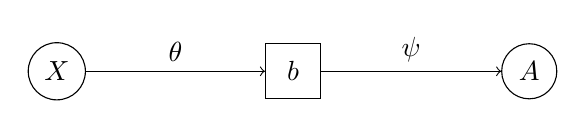
\begin{tikzpicture}[
		roundnode/.style={circle, draw=black, minimum size=7mm},
		squarednode/.style={rectangle, draw=black, minimum size=7mm}
		]
		% nodes
		\node[roundnode] (X) at (0, 0) {$X$};
		\node[squarednode] (b) at (3, 0) {$b$};
		\node[roundnode] (A) at (6, 0) {$A$};
		
		% arrows
		\draw[->] (X.east) -- node[above] {$\theta$} (b.west);
		\draw[->] (b.east) -- node[above] {$\psi$}(A.west);
	\end{tikzpicture}
	\caption{The feature-first block model (FFBM)}
	\label{fig:ffbm}
\end{figure}

Once the block memberships $b$ have been generated, we then draw the graph $A$ from the microcanonical DC-SBM (equation \ref{eqn:A-generation}) with additional parameters encapsulated by $\psi = \{\psi_e, \psi_k\}$.
%
\begin{equation}
	A \sim \textrm{DC-SBM}_{\textrm{MC}} (b, \psi_e, \psi_k)
	\label{eqn:A-generation}
\end{equation}


\subsection{Prior selection}

Before performing any inference, we must specify priors on $\theta$ and $\psi$. For $\theta$ it seems sensible to choose a Gaussian prior, with zero mean and variance matrix $\sigma^2_\theta I$ such that each element of $\theta$ is independent and distributed like $\sim \Gaussian(0, \sigma_\theta^2)$. In vector form, the prior for $\theta$ is therefore:
%
\begin{equation}
	p(\theta) = \Gaussian \left( \theta ; 0, \sigma_\theta^2 I \right)
	\label{eqn:theta-prior}
\end{equation}
%
In our model, the block memberships vector $b$ is an intermediate latent variable and so we are not free to choose a prior for it. Nevertheless, as far as inference on the right-hand-side of figure \ref{fig:ffbm}, we regard $p(b | X)$ as a pseudo-prior on $b$. We can show (appendix \ref{appdx:b|x}) that our choice of prior for $p(\theta)$ in equation \ref{eqn:theta-prior} leads to a uniform $p(b | X)$ in equation \ref{eqn:b-pseudo-prior}.
%
\begin{equation}
	p(b | X) = \int p(b | X, \theta) p(\theta) d\theta = B^{-N}
	\label{eqn:b-pseudo-prior}
\end{equation}
%
This is an enormously important simplification as evaluating $p(b | X)$ does not require an expensive Monte-Carlo integration over the $\theta$-domain nor does it require the exact value of $X$. \citet{Peixoto-Bayesian-Microcanonical} proposes careful choices for the additional microcanonical SBM parameters $\psi$ which we adopt. Peixoto's idea is to write the joint prior on $(b, e, k)$ as a product of conditionals $p(b, e, k) = p(b) p(e | b) p(k | e, b)= p(b) p(\psi | b)$. For our purposes we must insert a conditioning on $X$, to form our pseudo-prior for $b$ and $\psi$, to give equation \ref{eqn:joint-pseudo-prior}.
%
\begin{equation}
	p(b, \psi | X) = p(b | X) p(\psi | b, X) = p(b | X) p(\psi | b)
	\label{eqn:joint-pseudo-prior}
\end{equation}
%
Where we leverage the fact $(\psi \indep X) | b$. We then borrow the priors proposed by \citet{Peixoto-Bayesian-Microcanonical} for $p(\psi | b)$ to complete our model. Please refer to appendix \ref{appdx:sbm} for the exact form of $p(\psi | b)$. All that concerns the main argument is we have a computable form.

	%\subsection{Prior selection}

To complete the description of our Bayesian framework,
priors on $\theta$ and $\psi$ must also be specified. 
We place a Gaussian prior on $\theta$ such that
each element of $\theta$ has an independent ${\cal N}(0,\sigma_\theta^2)$
prior, with hyperparameter $\sigma_\theta^2$:
%
\begin{equation}
	p(\theta) \sim \mathcal{N} \left( \theta ; 0, \sigma_\theta^2 I \right).
	\label{eqn:theta-prior}
\end{equation}
%
This choice of prior gives a very
simple form for the conditional distribution of the block membership vector $b$ given $X$; it is a uniform distribution:
%
\begin{equation}
	p(b | X) = \int p(b | X, \theta) p(\theta) d\theta = B^{-N}.
	\label{eqn:b-pseudo-prior}
\end{equation}
%
The proof is given in Appendix~\ref{appdx:b|x}. This is an important simplification as evaluating $p(b | X)$ does not require an expensive  integration over $\theta$ nor does it depend on $X$.
Peixoto \cite{Peixoto-Bayesian-Microcanonical} proposes careful choices for 
the priors on the additional microcanonical SBM parameters $\psi$, which we adopt without repeating their exact form here. 
The idea is to write the joint distribution on $(b, e, k)$ as a product of 
conditionals, $p(b, e, k) = p(b) p(e | b) p(k | e, b)= p(b) p(\psi | b)$. 
In our case, conditioning on $X$ is also necessary, leading to,
$
p(b, \psi | X) = p(b | X) p(\psi | b, X) = p(b | X) p(\psi | b),
$
where we used the fact $\psi$ and $X$ are conditionally 
independent given $b$.
All that concerns the main argument is that $p(\psi|b)$ has
an easily computable form.
	
	\section{Inference}
\label{sec:inference}

Having completed the definition of the FFBM, we wish to leverage it 
to perform inference. Specifically, given a labelled network $(A, X)$, we wish to infer if and how the observed features $X$ impact the graphical structure $A$. Formally,
this means characterising the posterior distribution:
$
p(\theta|A, X) \propto p(\theta) \cdot p(A | X, \theta).
$
Although the prior is easily computable, 
computing the likelihood 
requires summing over all latent block-states, 
$p(A| X, \theta) = \sum_{b \in [B]^N} p(A | b) P(b | X, \theta)$, which is 
clearly impractical. In fact, this
approach is doubly intractable as we would also 
need to compute the normalising constant $p(A|X)$.
Therefore, following standard Bayesian practice,
instead we aim to draw samples from the posterior,
%
\begin{equation}
	\label{eqn:theta-target}
	\theta^{(t)} \sim p(\theta | A, X).
\end{equation}
%
We propose an iterative Markov chain Monte Carlo
(MCMC) approach to obtain these samples
$\{\theta^{(t)}\}$. We first draw a sample $b^{(t)}$ 
from the block membership posterior,
and then use $b^{(t)}$ to obtain a corresponding
sample $\theta^{(t)}$:
%
\begin{equation}
	b^{(t)} \stackrel{\rm distr}{\approx} p \big( b | A, X \big) 
	\quad \textrm{then} \quad
	\theta^{(t)} \stackrel{\rm distr}{\approx} 
	p\big(\theta | X, b^{(t)} \big),
\end{equation}
%
where these approximations become exact as
the number of MCMC iterations $t\to\infty$.
As described in the following subsections,
this can be implemented through a two-level
Markov chain via the Metropolis-Hastings (MH) 
algorithm \cite{hastings-alg}.
The splitting of the Markov chain into two levels allows us to side-step the summation over
all latent $b \in [B]^N$ required to directly compute the likelihood, $p(A| X, \theta)$.
The resulting $\theta^{(t)}$ samples are asymptotically
unbiased in that the expectation of 
their distribution converges to the true posterior:
%
\begin{equation}
\lim_{t\to\infty}
\Expect_{b^{(t)}} \left[p \left( \theta | X, b^{(t)} \right) \right] = \sum_{b \in [B]^N} p(\theta | X, b) p(b | A, X) = p(\theta | A, X).
\label{eqn:theta-unbiased}
\end{equation}
%
This is an example of a pseudo-marginal approach;
see, e.g., Andrieu and Roberts~\cite{pseudo-marginal} 
for a detailed rigorous derivation based on~(\ref{eqn:theta-unbiased}).
%
\begin{figure}[!ht]
	\centering

	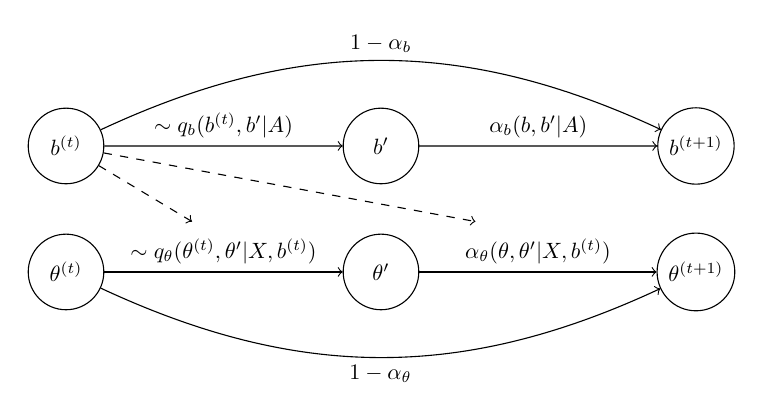
\begin{tikzpicture}[
		scale=0.8, every node/.style={transform shape},
		roundnode/.style={circle, draw=black, minimum size=12mm},
		squarednode/.style={rectangle, draw=black, minimum size=12mm}
		]
		% nodes
		\node[roundnode] (b0) at (0, 2) {$b^{(t)}$};
		\node[roundnode] (b1) at (5, 2) {$b'$};
		\node[roundnode] (b2) at (10, 2) {$b^{(t+1)}$};
		\node[roundnode] (t0) at (0, 0) {$\theta^{(t)}$};
		\node[roundnode] (t1) at (5, 0) {$\theta'$};
		\node[roundnode] (t2) at (10, 0) {$\theta^{(t+1)}$};
		
		% arrows
		\draw[->] (b0) to node[above] {$\sim q_b ( b^{(t)}, b' | A )$} (b1);
		\draw[->] (b1) to node[above] {$\alpha_b (b, b' | A )$} (b2);
		\draw[->] (b0) [out=25, in=155] to node[above] {$1-\alpha_b$} (b2);
		
		\draw[->] (t0) to node[above] {$\sim q_\theta(\theta^{(t)}, \theta' | X, b^{(t)})$} (t1);
		\draw[->] (t1) to node[above] {$\alpha_\theta (\theta, \theta' | X, b^{(t)})$} (t2);
		\draw[->] (t0) [out=-25, in=-155] to node[below] {$1-\alpha_\theta$} (t2);
		
		\draw[dashed, ->] (b0) to (2, 0.8);
		\draw[dashed, ->] (b0) to (6.5, 0.8);
		
	\end{tikzpicture}
	\caption{$\theta$-sample generation.}
	\label{fig:samp-sequence}
\end{figure}
 
Figure \ref{fig:samp-sequence} shows an overview of the proposed method, with $q$ and $\alpha$ denoting the MH proposal distribution and acceptance probability respectively.
Note the importance of the simplification in~(\ref{eqn:b-pseudo-prior}). 
As evaluating $p(b| X)$ does not depend on $X$, 
we do not need $X$ to sample $b$.
And on the other level, in order to obtain 
samples for $\theta$
we use only $b$ but not $A$, as $(\theta \indep A )| b$. 

\FloatBarrier
\subsection{Sampling block memberships}

To generate the required $b$-samples, we adopt the MCMC
procedure of
\cite{Peixoto-MCMC},
which relies on writing the posterior in the following form,
%
\begin{equation}
	p(b | A, X) \propto p(A | b, X) \cdot p(b | X) = \pi_b(b),
\end{equation}
%
where $\pi_b(\cdot)$ denotes the un-normalised target density.
Since we are using the microcanonical SBM formulation, there is only one 
value of $\psi$ that is compatible with the given $(A, b)$ pair;
recall the constraints in~(\ref{eqn:sbm-constraints}).
We denote this value $\psi^* = \{\psi_k^*, \psi_e^*\}$. Therefore, 
the summation over all $\psi$ needed to evaluate $p(A | b, X)$ reduces to just the single $\psi^*$ term:
$p(A | b, X) = \sum_{\psi} \nolimits p(A , \psi | b, X) = p(A, \psi^* | b, X)$.
In
this context, the microcanonical entropy of the configuration $b$
is,
%
\begin{equation}
	S(b) \coloneqq - \log \pi_b(b) = - \Big( \log p(A | b, \psi^*) + \log p(\psi^*, b | X) \Big),
	\label{eqn:dl-form}
\end{equation}
%
which can be thought of as the optimal
``description length'' of the graph. 
This expression will later be employed 
to help evaluate experimental results. 
The exact form of the proposal $q_b$ is explored thoroughly in
\cite{Peixoto-MCMC} and not repeated here. We use the \verb*|graph-tool| \cite{peixoto_graph-tool_2014}
library for Python, which implements this algorithm.
The only modification is in 
the prior $p(b)$ that we replace with $p(b|X)=B^{-N}$, 
which cancels out in the MH accept-reject step as it is independent of $b$.

\subsection{Sampling feature-to-block generator parameters}
\label{s:sfb}

The target distribution for the required $\theta$-samples 
is the posterior of $\theta$ given the values of the pair $(X, b)$. 
We write this as,
%
\begin{equation}
	\pi_\theta(\theta) \propto p(\theta | X, b) \propto p(b | X, \theta) p(\theta) \propto  \exp \left( - U(\theta) \right),
	\label{eq:U}
\end{equation}
%
where $U(\theta)$ denotes the negative log-posterior. Let $y_{ij} \coloneqq \one \left\{ b_i = j \right\}$ and $a_{ij} \coloneqq \phi_j(x_i; \theta)$. 
Discarding constant terms, $U(\theta)$ can be expressed as,
%
\begin{equation}
	U(\theta) = \left( \sum_{i \in [N]} \sum_{j \in [B]} y_{ij} \log \frac{1}{a_{ij}} \right)
	+ \frac{1}{2\sigma_\theta^2} \|\theta\|^2 = N \cdot \Lcal(\theta) + \frac{1}{2\sigma_\theta^2} \|\theta\|^2;
	\label{eqn:U-form}
\end{equation}
%
see Appendix \ref{appdx:form-U}. The function $U(\theta)$ is a typical objective function for neural network training. The first term $N \cdot \Lcal(\theta)$ is introduced by the likelihood and represents the cross-entropy between the graph-predicted and feature-predicted block memberships. 
The second term, introduced by the prior, brings a form of regularisation, guarding against over-fitting. In order to draw samples from the posterior 
$\pi_\theta \propto \exp(-U)$ we adopt the Metropolis-adjusted Langevin 
algorithm (MALA) \cite{mala-tweedie}, which uses $\nabla U$ to bias the 
proposal towards regions of higher density. Given the current 
sample $\theta$, a proposed 
new sample $\theta'$ is generated from,
%
\begin{equation*}
	\theta' \sim q_\theta\big(\theta, \theta'\big) 
	= \Gaussian \big( \theta' ; \theta - h \nabla U(\theta), 2h I \big),
\end{equation*}
%
where $\xi \sim \Gaussian(0, I)$ and $h$ is a step-size parameter 
which may vary with the sample index.
Without the injected noise term $\xi$, MALA is equivalent to gradient descent. We require $\xi$ to fully explore the parameter space. 
The term $\nabla U$ has an easy to compute analytic form (derived in Appendix \ref{appdx:form-U}).

\subsection{Sampling sequence}
\label{s:ss}

So far, each $\theta^{(t)}$ update has used its corresponding $b^{(t)}$ sample. This means the evaluation of $U^{(t)}$ and $\nabla U^{(t)}$ has high variance, leading to longer burn-in and possibly slower MCMC convergence. The only link between $b^{(t)}$ and $\theta^{(t)}$ is in the evaluation of $U^{(t)}$ and $\nabla U^{(t)}$ which depends only on the matrix $y^{(t)}$ with entries $y_{ij}^{(t)} \coloneqq \one\{b_i^{(t)} = j\}$. We would rather deal with the expectation of each $y_{ij}^{(t)}$:
%
\begin{equation}
	\Expect \left[ y_{ij}^{(t)} \right] = \Expect_{b^{(t)}} \left[ \one \left( b_{i}^{(t)} = j \right) \right]
	= p(b_i = j | A, X).
\end{equation}
%
An unbiased estimate for this can be obtained using 
the thinned $b$-samples after burn-in.
Let $\Tcal_b$  denote the retained set of indices 
for the $b$-samples and $\Tcal_\theta$ similarly for the $\theta$-chain. 
The unbiased estimate for $y_{ij}^{(t)}$ is then:
%
\begin{equation}
	\hat{y}_{ij} \coloneqq \frac{1}{|\Tcal_b|} \sum_{t \in \Tcal_b} y_{ij}^{(t)} = \frac{1}{|\Tcal_b|} \sum_{t \in \Tcal_b} \one\{b_i^{(t)} = j\}.
	\label{eqn:y-hat}
\end{equation}
%
The same matrix $\hat{y}$ is used in each $\theta^{(t)}$ update step.
This way, it is not necessary to run the $b$ and $\theta$ Markov chains 
concurrently. Instead, we run the $b$-chain to completion and use it 
to generate $\hat{y}$ also allowing us to vary the lengths of each.

\subsection{Dimensionality reduction}
\label{sec:dim-reduction}

The complexity of evaluating $U$ and $\nabla U$ is linear in 
the dimension of the feature space $D$,
so there is computational incentive to reduce $D$.
Given the samples $\left\{ \theta^{(t)} \right\}$, we can compute the empirical mean and standard deviation of each component of $\theta$. 
Switching to the matrix notation $W$ for $\theta$,
let:
%
\begin{equation}
	\hat{\mu}_{ij} \coloneqq \frac{1}{|\Tcal_\theta|} \sum_{t \in \Tcal_\theta} W_{ij}^{(t)} \qquad \textrm{and} \qquad
	\hat{\sigma}_{ij}^2 \coloneqq \frac{1}{|\Tcal_\theta|} \sum_{t \in \Tcal_\theta} \left( W_{ij}^{(t)} - \hat{\mu}_{ij} \right)^2.
\end{equation}
%
A simple heuristic to discard the least important features requires specifying a cutoff $c > 0$ and a multiplier $k > 0$. We define the function $\Fcal_i(j)$ 
as in~(\ref{eqn:fij}) and only keep features with indices $d \in \Dcal'$, where $\Dcal'$ is given in~(\ref{eqn:kept-feature-set}).
%
\begin{align}
	\Fcal_i(j) &\coloneqq (\hat{\mu}_{ij} - k \hat{\sigma}_{ij}, \hat{\mu}_{ij} + k \hat{\sigma}_{ij}) \cap (-c, +c),
	\label{eqn:fij} \\
	\Dcal' &\coloneqq \left\{ j \in [D] : \exists i \in [B] \textrm{ s.t. }  \Fcal_i(j) = \emptyset \right\}.
	\label{eqn:kept-feature-set}
\end{align}
%
Intuitively, this means discarding any feature $j$ for which 
$(\hat{\mu}_{ij} - k\hat{\sigma}_{ij}, \hat{\mu}_{ij} + k \hat{\sigma}_{ij})$ overlaps with
$(-c, c)$ for all $i$. If we were to use the Laplace approximation for the posterior $p(W_{ij} | A, X) \approx \Gaussian(W_{ij}; \hat{\mu}_{ij}, \hat{\sigma}_{ij}^2)$, then this would be analogous to a hypothesis test on the magnitude of $W_{ij}$ compared to $c$ with multiplier $k$ in~(\ref{eqn:fij}) determining the degree of significance of the result. Conversely, if we want to fix the number of dimensions in our reduced feature set $|\Dcal'|=D'$, the problem then becomes finding the largest value of $c$ such that $|\Dcal'|=D'$ given $k=k_0$:
%
\begin{equation}
	c^* = \argmax \{c>0\; : \;|\Dcal'| = D', k=k_0\}.
	\label{eqn:c-star}
\end{equation}


	\subsection{Sampling block memberships}

To generate the required $b$-samples, we adopt the MCMC
procedure of
\cite{Peixoto-MCMC},
which relies on writing the posterior in the following form,
%
\begin{equation}
	p(b | A, X) \propto p(A | b, X) \cdot p(b | X) = \pi_b(b),
\end{equation}
%
where $\pi_b(\cdot)$ denotes the un-normalised target density.
Since we are using the microcanonical SBM formulation, there is only one 
value of $\psi$ that is compatible with the given $(A, b)$ pair;
recall the constraints in~(\ref{eqn:sbm-constraints}).
We denote this value $\psi^* = \{\psi_k^*, \psi_e^*\}$. Therefore, 
the summation over all $\psi$ needed to evaluate $p(A | b, X)$ reduces to just the single $\psi^*$ term:
$p(A | b, X) = \sum_{\psi} \nolimits p(A , \psi | b, X) = p(A, \psi^* | b, X)$.
In
this context, the microcanonical entropy of the configuration $b$
is,
%
\begin{equation}
	S(b) \triangleq - \log \pi_b(b) = - \Big( \log p(A | b, \psi^*) + \log p(\psi^*, b | X) \Big),
	\label{eqn:dl-form}
\end{equation}
%
which can be thought of as the optimal
``description length'' of the graph. 
This expression will later be employed 
to help evaluate experimental results. 
The exact form of the proposal $q_b$ is explored thoroughly in
\cite{Peixoto-MCMC} and not repeated here. We use the \verb*|graph-tool| \cite{peixoto_graph-tool_2014}
library for Python, which implements this algorithm.
The only modification is in 
the prior $p(b)$ that we replace with $p(b|X)=B^{-N}$, 
which cancels out in the MH accept-reject step as it is independent of $b$.

\subsection{Sampling feature-to-block generator parameters}
\label{s:sfb}

The target distribution for the required $\theta$-samples 
is the posterior of $\theta$ given the values of the pair $(X, b)$. 
We write this as,
%
\begin{equation}
	\pi_\theta(\theta) \propto p(\theta | X, b) \propto p(b | X, \theta) p(\theta) \propto  \exp \left( - U(\theta) \right),
	\label{eq:U}
\end{equation}
%
where $U(\theta)$ denotes the negative log-posterior. Let $y_{ij} \triangleq \boldsymbol{1} \left\{ b_i = j \right\}$ and $a_{ij} \triangleq \phi_j(x_i; \theta)$. 
Discarding constant terms, $U(\theta)$ can be expressed as,
%
\begin{equation}
	U(\theta) = \left( \sum_{i \in [N]} \sum_{j \in [B]} y_{ij} \log \frac{1}{a_{ij}} \right)
	+ \frac{1}{2\sigma_\theta^2} \|\theta\|^2 = N \cdot \mathcal{L}(\theta) + \frac{1}{2\sigma_\theta^2} \|\theta\|^2;
	\label{eqn:U-form}
\end{equation}
%
see Appendix \ref{appdx:form-U}. The function $U(\theta)$ is a typical objective function for neural network training. The first term $N \cdot \mathcal{L}(\theta)$ is introduced by the likelihood and represents the cross-entropy between the graph-predicted and feature-predicted block memberships. 
The second term, introduced by the prior, brings a form of regularisation, guarding against over-fitting. In order to draw samples from the posterior 
$\pi_\theta \propto \exp(-U)$ we adopt the Metropolis-adjusted Langevin 
algorithm (MALA) \cite{mala-tweedie}, which uses $\nabla U$ to bias the 
proposal towards regions of higher density. Given the current 
sample $\theta$, a proposed 
new sample $\theta'$ is generated from,
%
\begin{equation*}
	\theta' \sim q_\theta\big(\theta, \theta'\big) 
	= \mathcal{N} \big( \theta' ; \theta - h \nabla U(\theta), 2h I \big),
\end{equation*}
%
where $\xi \sim \mathcal{N}(0, I)$ and $h$ is a step-size parameter 
which may vary with the sample index.
Without the injected noise term $\xi$, MALA is equivalent to gradient descent. We require $\xi$ to fully explore the parameter space. 
The term $\nabla U$ has an easy to compute analytic form (derived in Appendix \ref{appdx:form-U}).

\subsection{Sampling sequence}
\label{s:ss}

So far, each $\theta^{(t)}$ update has used its corresponding $b^{(t)}$ sample. This means the evaluation of $U^{(t)}$ and $\nabla U^{(t)}$ has high variance, leading to longer burn-in and possibly slower MCMC convergence. The only link between $b^{(t)}$ and $\theta^{(t)}$ is in the evaluation of $U^{(t)}$ and $\nabla U^{(t)}$ which depends only on the matrix $y^{(t)}$ with entries $y_{ij}^{(t)} \triangleq \boldsymbol{1}\{b_i^{(t)} = j\}$. We would rather deal with the expectation of each $y_{ij}^{(t)}$:
%
\begin{equation}
	\mathbb{E} \left[ y_{ij}^{(t)} \right] = \mathbb{E}_{b^{(t)}} \left[ \boldsymbol{1} \left( b_{i}^{(t)} = j \right) \right]
	= p(b_i = j | A, X).
\end{equation}
%
An unbiased estimate for this can be obtained using 
the thinned $b$-samples after burn-in.
Let $\mathcal{T}_b$  denote the retained set of indices 
for the $b$-samples and $\mathcal{T}_\theta$ similarly for the $\theta$-chain. 
The unbiased estimate for $y_{ij}^{(t)}$ is then:
%
\begin{equation}
	\hat{y}_{ij} \triangleq \frac{1}{|\mathcal{T}_b|} \sum_{t \in \mathcal{T}_b} y_{ij}^{(t)} = \frac{1}{|\mathcal{T}_b|} \sum_{t \in \mathcal{T}_b} \boldsymbol{1}\{b_i^{(t)} = j\}.
	\label{eqn:y-hat}
\end{equation}
%
The same matrix $\hat{y}$ is used in each $\theta^{(t)}$ update step.
This way, it is not necessary to run the $b$ and $\theta$ Markov chains 
concurrently. Instead, we run the $b$-chain to completion and use it 
to generate $\hat{y}$ also allowing us to vary the lengths of each.

\subsection{Dimensionality reduction}
\label{sec:dim-reduction}

The complexity of evaluating $U$ and $\nabla U$ is linear in 
the dimension of the feature space $D$,
so there is computational incentive to reduce $D$.
Given the samples $\left\{ \theta^{(t)} \right\}$, we can compute the empirical mean and standard deviation of each component of $\theta$. 
Switching to the matrix notation $W$ for $\theta$,
let:
%
\begin{equation}
	\hat{\mu}_{ij} \triangleq \frac{1}{|\mathcal{T}_\theta|} \sum_{t \in \mathcal{T}_\theta} W_{ij}^{(t)} \qquad \textrm{and} \qquad
	\hat{\sigma}_{ij}^2 \triangleq \frac{1}{|\mathcal{T}_\theta|} \sum_{t \in \mathcal{T}_\theta} \left( W_{ij}^{(t)} - \hat{\mu}_{ij} \right)^2.
\end{equation}
%
A simple heuristic to discard the least important features requires specifying a cutoff $c > 0$ and a multiplier $k > 0$. We define the function $\mathcal{F}_i(j)$ 
as in~(\ref{eqn:fij}) and only keep features with indices $d \in \mathcal{D}'$, where $\mathcal{D}'$ is given in~(\ref{eqn:kept-feature-set}).
%
\begin{align}
	\mathcal{F}_i(j) &\triangleq (\hat{\mu}_{ij} - k \hat{\sigma}_{ij}, \hat{\mu}_{ij} + k \hat{\sigma}_{ij}) \cap (-c, +c),
	\label{eqn:fij} \\
	\mathcal{D}' &\triangleq \left\{ j \in [D] : \exists i \in [B] \textrm{ s.t. }  \mathcal{F}_i(j) = \emptyset \right\}.
	\label{eqn:kept-feature-set}
\end{align}
%
Intuitively, this means discarding any feature $j$ for which 
$(\hat{\mu}_{ij} - k\hat{\sigma}_{ij}, \hat{\mu}_{ij} + k \hat{\sigma}_{ij})$ overlaps with
$(-c, c)$ for all $i$. If we were to use the Laplace approximation for the posterior $p(W_{ij} | A, X) \approx \mathcal{N}(W_{ij}; \hat{\mu}_{ij}, \hat{\sigma}_{ij}^2)$, then this would be analogous to a hypothesis test on the magnitude of $W_{ij}$ compared to $c$ with multiplier $k$ in~(\ref{eqn:fij}) determining the degree of significance of the result. Conversely, if we want to fix the number of dimensions in our reduced feature set $|\mathcal{D}'|=D'$, the problem then becomes finding the largest value of $c$ such that $|\mathcal{D}'|=D'$ given $k=k_0$:
%
\begin{equation}
	c^* = {\operatorname{argmax}} \{c>0\; : \;|\mathcal{D}'| = D', k=k_0\}.
	\label{eqn:c-star}
\end{equation}


	
	\section{Experiments}

We apply the developed methods to a variety of datasets, to show the power of the method across different scenarios. We choose datasets to span a range of node counts $N$, edge counts $E$ and feature space dimension $D$.

\begin{itemize}
	\item \textbf{Political books} \cite{polbooks} ($N=105, E=441, D=3$) - network of Amazon book sales about U.S. politics, published close to the presidential election in 2004. Two books are connected if they were frequently co-purchased by the same customer. Vertex features encode the broad political affiliation of the author (liberal, conservative or neutral).
		
	\item \textbf{Primary school dynamic contacts} \cite{schools} ($N=238, E=5539, D=13$) - network of face-to-face contacts amongst students and teachers at a primary school in Lyon, France. Two nodes are connected if the two parties shared a face-to-face interaction over the course of the day. Vertex features include class membership, gender and whether or not the individual is a teacher or pupil. These data were collected on consecutive days in October 2009. We choose to analyse just the second day.
	
	\item \textbf{Facebook egonet} \cite{fb-snap} ($N=747, E=30025, D=480$) - an assortment of Facebook egonets. These are networks of a particular user's friends list and all the connections within that. Vertex features are extracted from each user's profile and are fully anonymized. We focus on the egonet with id 1912.
	
%	\item \textbf{Maier Facebook Egonet} \cite{FB-Maier}  ($N=349, E=2336, D=32$) - egonet of the author's Facebook friends list. Each vertex has been manually labelled with a variety of features describing their relationship to the author. For our purposes we remove all nodes of degree 1 (those that are only connected to the egonode) as these cannot be said to be part of any community present in the graph.
%		
%	\item \textbf{Law firm} \cite{LawFirm} - a network of relationships between members of a law firm. Each relationship is categorised according to type: coworkers, friends or advice.
%	
%	\item \textbf{Twitch users} \cite{twitch} - a network of user-user friendships on the streaming service Twitch. Vertex labels are extracted according to video-games played, location and streaming habits. This dataset is also broken down into disjoint networks according to language. We only consider the English users with is a subnet with $N=7126$ vertices and $E=35324$ edges).

\end{itemize}

We require metrics to assess the relative model evidence for the FFBM. This can be split into two separate components: the microcanonical SBM fit (concerned with the $b$-samples) and the fit of the feature-to-block generator (concerned with the $\theta$-samples). For each of these we can evaluate the mean of the unnormalised log-target of each Markov chain.
%
\begin{equation}
	\bar{S}_b \coloneqq \frac{1}{T_b} \sum_{t=1}^{T_b} S \left( b^{(t)} \right) \qquad \textrm{and} \qquad
	\bar{U}_\theta \coloneqq \frac{1}{T_\theta} \sum_{t=1}^{T_\theta} U \left( \theta^{(t)} \right)
\end{equation}
%
The lower these quantities, the better the fit of each stage of the model. To allow for rough comparison between datasets, we divide these quantities by the number of vertices in the graph $N$. Table \ref{tab:results} summarises the results for each experiment.

\begin{table}[!h]
	\centering
	\caption{FFBM fit for the datasets}
	\label{tab:results}
	\begin{tabular}{c|ccc|c|cc}
		Dataset & $N$ & $E$ & $D$ & $B$ & $\bar{S}_b /N$ & $\bar{U}_\theta /N$ \\ \hline
		Political books & 105  & 441 & 3 & 3 & 11.7 & 0.707 \\
		Primary school & 238 & 5539 & 13 &  10 & 45.9  & 1.61 \\
		FB egonet & 747 & 30025 & 480 & 10  & 66.9 & 7.47
	\end{tabular}
\end{table}

\FloatBarrier
\subsection{Political books}

This dataset was collected by \citet{polbooks}. We wish to determine whether political affiliation is a good predictor of the overall network structure. We choose to partition the network into $B=3$ communities as we only have this many distinct values for political affiliation (conservative, liberal or neutral). The inferred block memberships are given in figure \ref{fig:books-graph}. We sample the block-generator parameters and plot the emprical mean and standard deviation of each sample on figure \ref{fig:book-null}.
%
\begin{figure}[!h]
	\centering
	\begin{subfigure}{0.3\linewidth}
		\centering
		\includegraphics[width=\linewidth]{polbooks-graph.png}
		\fbox{\includegraphics[width=0.4\linewidth]{3-legend.png}}
		\caption{Sampled block memberships $\hat{Y}$}
		\label{fig:books-graph}
	\end{subfigure}
	\hfill
	\begin{subfigure}{0.5\linewidth}
		\centering
		\includegraphics[width=\linewidth]{polbooks-null.png}
		\caption{Feature weights}
		\label{fig:book-null}
	\end{subfigure}
	\caption{Political books network \cite{polbooks}}
\end{figure}
%
Indeed, for all 3 blocks, each has a distinct political affiliation as its highest magnitude component. This is strong evidence that political affiliation is indeed the axis which best predicts the 3-way natural partition of the graph into blocks. Nevertheless, for block index 1, although \verb*|neutral| is the best predictor of the ones we have available, the value is not particularly extreme. Perhaps, there is an unobserved feature that places a book into this block. Indeed, block-0 is more of a centre-right block than true centre.

\FloatBarrier
\subsection{Primary school dynamic contacts}

These data were originally collected by \citet{schools} to quantify the transmission opportunities for respiratory infections. However, we seek to ask which vertex features best describe how people interact with one another in a primary school context. The only vertex features we have available are school-class (one of 10 values - 2 per year group), gender and a distinction between teachers and pupils.

We must first choose the number of blocks $B$ to define the coarseness of our analysis. A total of 10 school-classes would suggest that $B=10$ is a natural starting point. We visualise the inferred block memberships in figure \ref{fig:school-graph}.
%
\begin{figure}[!h]
	\centering
	\begin{subfigure}{0.45\linewidth}
		\centering
		\includegraphics[width=\linewidth]{school-graph.png}
		\fbox{\includegraphics[width=0.5\linewidth]{10-legend.png}}
		\caption{Sampled block memberships $\hat{Y}$}
		\label{fig:school-graph}
	\end{subfigure}
	\hfill
	\begin{subfigure}{0.45\linewidth}
		\centering
		\includegraphics[width=\linewidth]{school-null.png}
		\caption{Reduced dimension feature weights}
		\label{fig:school-null}
	\end{subfigure}
	\caption{Primary school dynamic contacts network \cite{schools}}
\end{figure}

As before, we proceed to sample the block-generator parameters $\theta$ and employ the dimensionality reduction heuristic defined in section \ref{sec:dim-reduction} with null threshold $c=1$ and standard deviation multiplier $k=1$. We then plot the weights for the features that survive the discard step in figure \ref{sec:dim-reduction}. Immediately, we see that only the pupils' class memberships have survived (1A-5B); gender and teacher/student status have been discarded meaning that these are not good predictors of overall macro-structure.

The vast majority of blocks are composed of a single class. However, some blocks have 2 comparably good classes as their predictor. For example, blocks 2 and 4 contain classes 4A and 4B as their 2 best predictors. This suggests that the social divide between classes is less pronounced for pupils in year 4 but there is nonetheless an unobserved variable that splits year 4 into 2 communities. The most surprising block is number 5 - which has comparable weightings for classes 5A and 1B. Perhaps there was a joint event between those two classes on the day the data were collected.

\subsection{Facebook egonet}

This dataset was chosen to showcase the power of the dimensionality reduction technique as the feature-space has high dimension ($D=480$). We sample the $b$-chain specifying $B=10$ total blocks and use this to construct the $\theta$-samples as before. 

We apply the dimensionality reduction heuristic outlined in section \ref{sec:dim-reduction}, choosing $k=1$ and $c=0.8$. This leads to a reduced dimension $D'=13$. These parameter values are plotted on figure \ref{fig:fb-null}. The features that remain are those that best explain the high-level community structure. More so than language, gender or surname - the school\footnote{This includes higher education institutes} you attend is the best explanatory variable for how the observed network's communities are partitioned at the highest level. 
%
\begin{figure}[!h]
	\centering
	\begin{subfigure}{0.45\linewidth}
		\centering
		\includegraphics[width=\linewidth]{fb-graph.png}
		\fbox{\includegraphics[width=0.3\linewidth]{10-legend.png}}
		\caption{Sampled block memberships $\hat{Y}$}
		\label{fig:fb-graph}
	\end{subfigure}
	\hfill
	\begin{subfigure}{0.45\linewidth}
		\centering
		\includegraphics[width=\linewidth]{fb-null.png}
		\caption{Reduced dimension feature weights}
		\label{fig:fb-null}
	\end{subfigure}
	\caption{Facebook egonet id 1912 \cite{fb-snap}}
\end{figure}

Nevertheless, this example also highlights a weakness of the method for high-dimensional feature spaces. When the feature dimension is very large, it becomes increasingly likely that a particular feature may uniquely identify a small set of nodes. If these nodes are all part of the same community then the classifier will overfit for that particular parameter. The regularisation term imposed by the prior goes some way to alleviating this problem but we see in figure \ref{fig:fb-null} that the feature \verb*|birthday-5| has a very high weight as it relates to block 0. It might be possible to shift the feature values such that they take values in $\{-1, 1\}$ rather than $\{0, 1\}$ but this approach falls down when input features are mutually correlated. Indeed, for features with discrete values such as the class memberships (1A, 1B, 2A \dots 5B) it is preferred to keep $x_i \in \{0, 1\}^D$ as then each block can be readily accept more than one mutually exclusive feature-group (i.e. two school-classes are part of the same block).


	\begin{table}[!h]
	\centering
	\caption{Experimental results averaged over $n=10$ iterations (mean $\pm$ std. dev.).}
	\label{tab:results}
	\resizebox{\textwidth}{!}{%
		\begin{tabular}{c|ccc|c|cc|ccc}
			Dataset  & $B$ & $D$ & $D'$ & $\bar{S}_e$ & $\bar{\Lcal}_0$ & $\bar{\Lcal}_1$ & $c^*$ & $\bar{\Lcal}_0'$ & $\bar{\Lcal}_1'$  \\ \hline
			Polbooks & 3 & 3 & -- & $2.250 \pm 0.000$ & $0.563 \pm 0.042$ & $0.595 \pm 0.089$ & -- & -- & -- \\
			School & 10 & 13 & 10 & $1.894 \pm 0.004$ & $0.787 \pm 0.127$ & $0.885 \pm 0.129$ & $1.198 \pm 0.249$ & $0.793 \pm 0.132$ & $0.853 \pm 0.132$ \\
			FB egonet & 10  & 480 & 10 & $1.626 \pm 0.003$ & $1.326 \pm 0.043$ & $1.538 \pm 0.069$ & $0.94 \pm 0.019$ & $1.580 \pm 0.150$ & $1.605 \pm 0.106$
		\end{tabular}
	}
\end{table}

\begin{figure}[!h]
	\centering
	\begin{subfigure}[t]{0.28\linewidth}
		\centering
		\includegraphics[width=\linewidth]{polbooks-graph.png}
		\caption{Polbooks}
		\label{fig:polbooks-graph}
	\end{subfigure}
	\hfill
	\begin{subfigure}[t]{0.28\linewidth}
		\centering
		\includegraphics[width=\linewidth]{school-graph.png}
		\caption{School}
		\label{fig:school-graph}
	\end{subfigure}
	\hfill
	\begin{subfigure}[t]{0.28\linewidth}
		\centering
		\includegraphics[width=\linewidth]{fb-graph.png}
		\caption{Facebook egonet}
		\label{fig:fb-graph}
	\end{subfigure}
	\begin{subfigure}[t]{0.11\linewidth}
		\centering
		\includegraphics[width=0.8\linewidth]{10-vertical-legend.png}
		\caption{Block Legend}
		\label{fig:10-legend}
	\end{subfigure}
	\caption{Networks laid out and coloured according to inferred block memberships $\hat{y}$ for a given experiment iteration. Visualisation performed using \textit{graph-tool} \cite{peixoto_graph-tool_2014}.}
	\label{fig:graphs-all}
\end{figure}


\begin{figure}[!h]
	\centering
	\begin{minipage}{0.42\linewidth}
		\centering
		\begin{subfigure}{\linewidth}
			\centering
			\imagebox{0.8\linewidth}{\includegraphics[width=\linewidth]{polbooks-null-1}}
			\caption{Political Books.}
			\label{fig:polbooks-null}
		\end{subfigure}
		
		\begin{subfigure}{\linewidth}
			\centering
			\imagebox{0.85\linewidth}{\includegraphics[width=\linewidth]{school-null-1}}
			\caption{Primary School.}
			\label{fig:school-null}
		\end{subfigure}
		
		\begin{subfigure}{\linewidth}
			\centering
			\imagebox{0.9\linewidth}{\includegraphics[width=\linewidth]{fb-null-1}}
			\caption{Facebook Egonet.}
			\label{fig:fb-null}
		\end{subfigure}
		\caption{$\theta$-samples. Dotted line $\pm c^*$.}
	\end{minipage}
	%
	\begin{minipage}{0.42\linewidth}
		\centering
		\begin{subfigure}[t]{\linewidth}
			\centering
			\imagebox{0.8\linewidth}{\includegraphics[width=\linewidth]{polbooks-accuracy-2}}
			\caption{Political Books.}
			\label{fig:polbooks-accuracy}
		\end{subfigure}
		
		\begin{subfigure}{\linewidth}
			\centering
			\imagebox{0.85\linewidth}{\includegraphics[width=\linewidth]{school-accuracy-1}}
			\caption{Primary School.}
			\label{fig:school-accuracy}
		\end{subfigure}
		
		\begin{subfigure}{\linewidth}
			\centering
			\imagebox{0.9\linewidth}{\includegraphics[width=\linewidth]{fb-accuracy-1}}
			\caption{Facebook Egonet.}
			\label{fig:fb-accuracy}
		\end{subfigure}
		\caption{Per-block accuracy $\eta(j)$.}
	\end{minipage}
\end{figure}
	%\begin{figure}[!ht]
	\centering
	\begin{subfigure}{0.32\linewidth}
			\centering
			\imagebox{0.9\linewidth}{\includegraphics[width=\linewidth]{polbooks-null-1}}
			\caption{Political books}
			\label{fig:polbooks-null}
		\end{subfigure}
	\begin{subfigure}{0.32\linewidth}
			\centering
			\imagebox{0.9\linewidth}{\includegraphics[width=\linewidth]{school-null-1}}
			\caption{Primary school}
			\label{fig:school-null}
		\end{subfigure}
	\begin{subfigure}{0.32\linewidth}
			\centering
			\imagebox{0.9\linewidth}{\includegraphics[width=\linewidth]{fb-null-1}}
			\caption{Facebook egonet}
			\label{fig:fb-null}
		\end{subfigure}
	\caption{Top $D'$ $\theta$-samples for each dataset. Coarse steps on x-axis give block index and the fine steps denote give index. Dotted line is $\pm c^*$.}
\end{figure}
%
\begin{figure}[!ht]
	\centering
	\begin{subfigure}{0.32\linewidth}
			\centering
			\imagebox{0.8\linewidth}{\includegraphics[width=\linewidth]{polbooks-accuracy-2}}
			\caption{Political books}
			\label{fig:polbooks-accuracy}
		\end{subfigure}
	\begin{subfigure}{0.32\linewidth}
			\centering
			\imagebox{0.8\linewidth}{\includegraphics[width=\linewidth]{school-accuracy-1}}
			\caption{Primary school}
			\label{fig:school-accuracy}
		\end{subfigure}
	\begin{subfigure}{0.32\linewidth}
			\centering
			\imagebox{0.8\linewidth}{\includegraphics[width=\linewidth]{fb-accuracy-1}}
			\caption{Facebook egonet}
			\label{fig:fb-accuracy}
		\end{subfigure}
	\caption{Per-block accuracy $\eta(j)$ for each dataset.}
\end{figure}
	%Table~\ref{tab:results} summarises the results for each experiment. We also apply the 
dimensionality reduction method 
of Section~\ref{sec:dim-reduction}
to the two higher dimensional datasets (the school and FB egonet). 
For this we use equation~(\ref{eqn:c-star}) with $k=1$,
in order to reduce the dimension from 
$D$ to a desired $D'$. 
We then retrain the feature-block predictor using only the retained 
feature set $\Dcal'$, and report the log-loss over the training and 
test sets for the reduced classifier -- 
denoted $\bar{\Lcal}_0'$ and $\bar{\Lcal}_1'$ respectively. 
These values are also given in Table~\ref{tab:results}.

Based on these results, some remarks are in order.
Firstly, the variance of the test loss $\bar{\Lcal}_1$ tends to be higher 
than the training loss $\bar{\Lcal}_0$. This is expected,
as the test set is smaller than the training set and hence 
more susceptible to variability in its construction. 
Secondly, it can be seen that the dimensionality reduction procedure 
brings the training and test losses closer together. This implies that 
the features we keep are indeed correlated with the underlying graphical 
partition and that the approach generalises correctly.

The average description length per entity,
$\bar{S}_e$, of the graph, 
has very small variance, suggesting that
the detected communities can be found reliably (to within an arbitrary 
relabelling of blocks). For reference, we plot an inferred partition for each 
of the graphs in Figure~\ref{fig:graphs-all}. The polbooks graph yields the cleanest separation between blocks but nonetheless the inferred partitions for the other datasets do succeed at dividing the graph into densely connected clusters.

\subsubsection{Political books}

\cite{polbooks} ($N=105, E=441, D=3$) -- network of Amazon political book sales, published close to the 2004 presidential election. Two books are connected if they were frequently co-purchased. Vertex features encode the political affiliation of the author (liberal, conservative, or neutral).

We choose to partition the network into $B=3$ communities as we only have this many distinct values for political affiliation (conservative, liberal or neutral).
From Figure~\ref{fig:polbooks-null} we see that all 3 blocks have a distinct political affiliation as their largest positive component.  
Furthermore, in Table~\ref{tab:results} we see that the training and test losses 
are very similar and both are low in magnitude. This is strong evidence 
that political affiliation is a very appropriate explanatory 
variable for the overall network structure.

However, from Figure~\ref{fig:polbooks-accuracy} we see that block 1 has low accuracy. 
This suggests that detected block 1 is not solely composed of ``neutral" books but also 
contains some ``liberal" and ``conservative" authors. Examining 
Figure~\ref{fig:polbooks-graph}, we see the majority of paths between blocks 2 and 3 go through block 1.
Block 1 is in effect a bridge between the ``conservative'' and ``liberal'' blocks so it is unsurprising that some books from either side leak into block 1.

\subsubsection{Primary school dynamic contacts}

\cite{schools} ($N=238, E=5539, D=13$) -- network of face-to-face contacts amongst students and teachers at a primary school in Lyon, France. Vertex features include class membership (one of 10 values: 1A-5B), gender (male, female) and teacher status encoded as an 11th school-class. We choose to analyse just the second day of results.

We choose the number of communities $B=10$, in line with the total number of 
school classes. From Figure~\ref{fig:school-null}, we see only the pupils' class memberships (1A-5B) have survived
the dimensionality-reduction process for $D'=10$;
gender and teacher/student status have been discarded,
meaning these are poor predictors of overall macro-structure.

The vast majority of blocks are composed of a single class. 
However, some blocks have two comparably strong classes as their predictors. 
For example, blocks 2 and 5 both contain classes 3A and 3B as their 2 best predictors. 
This suggests that the social divide between classes is less pronounced 
for pupils in year 3. Conversely, some classes are found to extend over two 
detected blocks (class 2B spans blocks 8 and 9) but we do 
not have a feature which explains the division.

Figure~\ref{fig:school-accuracy} shows excellent accuracy for the majority of blocks. In fact the only blocks with low accuracy are those that have a school-class span two blocks such that we cannot reliably distinguish between the two. This is more pronounced when we apply hard classification rather than the soft cross-entropy loss. Indeed block 1 has low accuracy because class 1A has a higher weight component for block 3 than it does for block 1. As we use hard classification to compute accuracy, vertices belonging to class 1A are predicted to belong to block 3. A similar effect is seen in block 5 which often loses out to block 2. The same can be said of blocks 8 and 9. However, in this case the weights for class 2B are very similar -- thus explaining the roughly evenly split accuracy for blocks 8 and 9.

\subsubsection{Facebook egonet}

\cite{fb-snap} ($N=747, E=30025, D=480$) -- an assortment of Facebook users' friends lists. Vertex features are fully anonymised and encode information about each user's education history, languages spoken, gender, home-town, birthday etc. We focus on the egonet with id 1912.

We choose $B=10$ and $D'=10$ for this experiment. The selected features 
(Figure~\ref{fig:fb-null}) are those that best explain the high-level 
community structure. The majority of them are education related. 
Nevertheless, for $D'=10$ we only have good explanations for some of the detected blocks; several blocks in 
Figure~\ref{fig:fb-null} do not have high-magnitude components for $D'=10$. This is further emphasised by the disparate accuracies in Figure~\ref{fig:fb-accuracy}. Nevertheless, observe that the accuracy is only high for blocks that contain high magnitude weights. The only exception to this rule is block 9 which nonetheless may have high magnitude weights just below the cut-off $c^*$.

When the feature dimension is very large, it becomes increasingly likely that 
a particular feature may uniquely identify a small set of nodes. If these nodes 
are all part of the same community, then the classifier may overfit for that 
particular parameter. The regularisation term imposed by the prior goes some 
way towards alleviating this problem. Nevertheless, we see in 
Figure~\ref{fig:fb-null} that the feature \verb*|birthday-5| has a very 
high weight as it relates to block 1 -- but it is highly unlikely
that birthdays determine graphical structure.
	
	%\section{Extensions}

The greatest limitation of the current FFBM formulation is that it can only explain structure at the macro-scale. In other words, we cannot explain structure within each detected block. Future work will benefit from extending the FFBM to be hierarchical in nature. This would be a relatively natural extension. Indeed, the SBM has already been extended to a hierarchical form, often called the nested SBM \cite{SBM-hierarchical}. The idea is to divide each block into sub-blocks and so on recursively until a specified depth is reached. The full block membership for a particular vertex now encodes the memberships at all levels of the hierarchy.

The necessary modification of the feature-to-block generator is also rather natural. Given the nested SBM, we would have a hierarchy of generators, each generating a block membership at a particular level of the hierarchy. Nevertheless, this does pose some practical issues for scalability; supposing we have $L$ levels in our hierarchy and each divides the parent block into $B$ sub-blocks, then the number of distinct generators necessary scales as $O(B^L)$. To avoid exponential growth in the number of model parameters, we could apply some form of dimensionality reduction as we descend the layers so that each generator is only given relevant features as input.
	\section{Conclusion}
\label{sec:conclusion}

An efficient MCMC algorithm 
is developed for sampling 
from the posterior distribution of
the relevant parameters in the FFBM;
the main idea is to divide up the graph into 
its most natural partition under the associated
parameter values, and then to determine whether 
the vertex features can accurately explain the partition. 
Through several applications on empirical
network data, this approach 
is shown to be effective at extracting and describing 
the most natural communities in a labelled network. 
Nevertheless, it
can only currently explain the structure at the macroscopic
scale. Future work will benefit from extending 
the FFBM to a further hierarchical model,
so that
the structure of the network 
can be explained at all scales of interest.



	
	% References should be placed in the text in author (year) form.
% The list of references should be placed below IN ALPHABETICAL ORDER.
% (Please follow the format of the examples very tightly).

\references
\begin{description}
	
	\item[Krebs, V.] (2004) . The political books network,
	http://www.orgnet.com/.

	\item[Leskovec, J., Mcauley, J.] (2012).
	Learning to discover social circles in ego networks.
	{\it Advances in Neural Information Processing Systems} vol. 25

	\item[Peixoto, T.P.] (2017).
	Nonparametric Bayesian inference of the microcanonical
	stochastic block model. Physical Review E 95(1).

	\item[Stanley, N. et al] (2019). Stochastic block models with multiple continuous attributes. Applied Network Science, 4(1), 1-22.

	\item[Stehle, J. et al] (2011).
	High resolution measurements of face-to-face contact patterns in a primary school.
	PLoS ONE 6(8), 1–-13.

	\item[Tray, L., Kontoyiannis, I.] (2021).
	The feature-first block model.
	arXiv preprint 2105.13762 [cs.LG].

\end{description}

	
\end{document}
